\ifx\inkludert\undefined
\input{preamble}
\usepackage{xr}
\externaldocument{lin-alg}
\newcommand{\kapittel}[2]{\setcounter{chapter}{#1}\addtocounter{chapter}{-1}\chapter{#2}}
\newcommand{\kapittelslutt}{\enddocument}
\begin{document}
\chapterstyle{tma4110}
\pagestyle{plain}
\fi


\kapittel{10}{Komplekse tall}
\label{ch:komplekse-tall}

Oppfinnelsen av nye tallsystemer henger gjerne sammen med løsning av polynomlikninger. Likningen 
\[
2x+4=0
\]
har ingen positiv løsning, selv om koeffisientene er positive tall. 
likningen
\[
2x-3=0
\]
har ingen heltallig løsning, selv om koeffisientente er hele tall.
likningen
\[
x^2-2=0
\]
har ingen rasjonale løsninger, siden
\[
x=\sqrt{2}
\]
ikke kan skrives som en brøk. 

Generelt er det slik at en polynomlikning
\[
a_nx^n+a_{n-1}x^{n-1}+...+a_1x+a_0=0
\]
ikke nødvendigvis har en løsning i det tallsystemet koeffisientene er hentet fra. 
Man kan spørre seg hvorvidt det finnes tallsystemer der en vilkårlig polynomlikning alltid har løsning, 
og svaret er ja. 
Vi skal ta for oss et slikt tallsystem, nemlig de \defterm{komplekse tallene}.
%Likningen 
%\[
%x^2+1=0
%\]
%ingen reelle løsninger. Hva gjør vi med det?


\section*{Den imaginære enheten}
For å komme igang med komplekse tall, kan vi betrakte likningen
\[
x^2+1=0.
\]
På gymnaset ville du sagt at denne likningen ikke har noen løsning, for det finnes ingen relle tall som passer i likningen. 

Derfor finner vi opp et nytt tall. Vi kaller det $i$, den \emph{den imaginære enheten}. 
Nå kan det være fristende å 'løse' likningen over for $x$, og definere
\[
i=\sqrt{-1}.
\]
Med dette nye tallet kan vi skrive kvadratroten av negative tall på en pen måte:
\begin{equation*}
\sqrt{-4}=\sqrt{4\cdot (-1)}=\sqrt{4}\cdot \sqrt{(-1)}=2i.
\end{equation*}
Men vi må være litt forsiktige med denne strategien. 
Regneregelen
\[
\sqrt{ab}=\sqrt{a}\sqrt{b}
\]
gjelder nemlig ikke når $a$ og $b$ er negative tall.
Følgende klassiske eksempel er litt artig:
\begin{align*}
1&=(-1)\cdot(-1)\\&=\sqrt{(-1)\cdot (-1)}\\&=\sqrt{-1}\cdot \sqrt{ -1}=i^2=-1.
\end{align*}

Med andre ord må vi være litt forsiktige med å sjonglere med negative tall og rottegn.
En god strategi er å definere $i$ ved likningen
\[
i^2=-1,
\]
for dette er egenskapen vi er ute etter. 
Skulle vi slumpe til å ta roten av et negativt tall, 
forter vi oss bare med å skrive det ved hjelp av den imaginære enheten, 
slik at vi ikke blir forledet til å utføre noen ulovlige regneoperasjoner.

\begin{ex}
Løser vi likningen
\[
x^2+x+1=0
\]
gir annengradsformelen
\[
x=\frac{-b\pm\sqrt{b^2-4ac}}{2a}
\]
at
\[
x=\frac{-1\pm\sqrt{-3}}{2}=-\frac{1}{2}\pm\frac{\sqrt{3}}{2}i. \qedhere
\]
\end{ex}

Eksemplet over inspirerer oss til å definere \emph{komplekse tall} som 
\[
z=a+bi.
\]
Her er $a$ og $b$ reelle tall. 
De kalles henholdsvis \emph{realdelen} og \emph{imaginærdelen} til $z$,
og skrives gjerne $\Re z$ og $\Im z$. 
Mengden av alle komplekse tall skrives $\C$. 
De reelle tallene er en delmengde av de komplekse tallene,% $\R \subset \C$, 
for dersom $b=0$, er $z$ reell. 

Et komplekst tall har en viss ytre likhet med vektorer i $\R^2$. 
Hvis komponentene til $\V x$ er $x_1$ og $x_2$, og enhetsvektorer i koordinatretningene er 
\[
\V{e}_1=\vv{1}{0} \quad \text{og} \quad \V{e}_2=\vv{0}{1}, 
\]
skriver vi gjerne
\[
\V{x}=x_1 \V{e}_1+x_2 \V{e}_2.
\]
På lignende vis kan vi tenke at realdelen $a$ og imaginærdelen $b$ er komponenter i en vektor,
%\[
%z=a+bi,
%\] 
og avmerke $z$ i \emph{det komplekse planet}. 
\begin{center}
\begin{tikzpicture}[scale=.42]
\draw[->] (-4,0) -- (7,0);
\draw[->] (0,-4) -- (0,6);
\node[anchor=east] at (9.8,0) {\footnotesize $\Re z$};
\node[anchor=south] at (0,6.8) {\footnotesize $\Im z$};
\foreach \x in {-4,-3,-2,-1,1,2,3,4,5,6}
\draw (\x,5pt) -- (\x,-5pt);
\foreach \y in {-4,-3,-2,-1,1,2,3,4,5}
\draw (5pt,\y) -- (-5pt,\y);
\filldraw (2,3) circle [radius=3pt] node[anchor=west] {$z=2+3i$};
\filldraw (2,-3) circle [radius=3pt] node[anchor=west] {$\overline z=2-3i$};
\filldraw (4,5) circle [radius=3pt] node[anchor=west] {$w=4+5i$};
%\filldraw (0,1) circle [radius=3pt] node[anchor=east] {$\V{e}_2$};
%\filldraw (-1,-2) circle [radius=3pt] node[anchor=east] {$\V{u}$};
%\filldraw (3,2) circle [radius=3pt] node[anchor=east] {$\V{v}$};
%\filldraw (1,4) circle [radius=3pt] node[anchor=south] {$A \V{e}_1$};
%\filldraw (3,-3) circle [radius=3pt] node[anchor=north] {$A \V{e}_2$};
%\filldraw (-7,2) circle [radius=3pt] node[anchor=east] {$A \V{u}$};
%\filldraw (9,6) circle [radius=3pt] node[anchor=north] {$A \V{v}$};
%\draw[->,shorten <=4pt,shorten >=4pt] (1,0) to[bend right=20] (1,4);
%\draw[->,shorten <=4pt,shorten >=4pt] (0,1) to[bend right=30] (3,-3);
%\draw[->,shorten <=4pt,shorten >=4pt] (-1,-2) to[bend right=20] (-7,2);
%\draw[->,shorten <=4pt,shorten >=4pt] (3,2) to[bend left=20] (9,6);
\end{tikzpicture}
\\
{\small \textit{Det komplekse planet}}
\end{center}
%Nå tenker du sikkert at det er på sin plass å sjekke om vektorromsaksiomene holder for de komplekse tallene. 
%Det er en helt riktig ting å gjøre, $\C$ er et vektorrom, 
%og de vanlige geometriske operasjonene man gjør på vektorer i $\R^2$, 
%fungerer fint på komplekse tall. 



\section*{Operasjoner på komplekse tall}
Regneregler for komplekse tall følger regnereglene for reelle tall, 
men du må huske at $i^2=-1$. 
\begin{tcolorbox}
\begin{thm}
La $z=a+bi$ og $w=c+di$ være komplekse tall. Vi har  
\begin{align*}
z+w&=a+c+(b+d)i \\[4pt]
z-w&=a-c+(b-d)i \\[4pt]
z\cdot w&=ac-bd+(bc+ad)i\\[4pt]
\frac{z}{w}&=\frac{ac+bd+(bc-ad)i}{c^2+d^2}
\end{align*}
\end{thm}
\vspace{1mm}
\end{tcolorbox}
\begin{proof}
De to første er trivielle. Vi beviser gangeregelen:
\begin{align*}
z\cdot w&=(a+bi)(c+di)\\
&= ac+bci+adi+bdi^2\\ 
&=ac-bd+(bc+ad)i
\end{align*}
og deleregelen:
\begin{align*}
\frac{z}{w}&=\frac{a+bi}{c+di}= \frac{a+bi}{c+di}\cdot \frac{c-di}{c-di}\\[4pt]
&=\frac{ac+bd+(bc-ad)i}{c^2+d^2} \qedhere
\end{align*}
\end{proof}

Komplekse tall legges altså sammen komponentvis akkurat som vektorer i $\R^2$, 
mens multiplikasjon og divisjon har ingen tilsvarende operasjoner i $\R^2$.


\begin{ex}
La $z=2+3i$ og $w=4+5i$. 
\begin{align*}
z+w&=2+4+(3+5)i=6+8i \\[7pt]
z-w&=2-4+(3-5)i=-2-2i \\[7pt]
z\cdot w&=(2+3i)\cdot(4+5i)\\&=2\cdot 4+3\cdot 4i+2\cdot 5i+3\cdot 5 i^2\\&=8-15+(12+10)i=-7+22i.\\[7pt]
\frac{z}{w}&=\frac{2+3i}{4+5i}=\frac{2+3i}{4+5i}\cdot\frac{4-5i}{4-5i}\\&=\frac{8+15+(12-10)i}{16+25}=\frac{22}{41}-\frac{2}{41}i. \qedhere
\end{align*}
\end{ex}
Når vi deler et komplekst tall på $z=a+bi$, 
ganger vi oppe og nede med \emph{$w$ konjugert}
\[
\overline z =a-bi.
\]
Merk at $z\overline z=a^2+b^2$ er et reelt tall.
Her  er et par regneregler for konjugering.
\begin{tcolorbox}
\begin{thm}
La $z=a+bi$ og $w$ være komplekse tall. Noen regneregler er:
\begin{align*}
\overline{z+w}&=\overline{z} + \overline{w} \hspace{.8cm}
\overline{z-w}=\overline{z} - \overline{w} \\
\overline{z\cdot w}&=\overline{z} \cdot \overline{w} \hspace{1.25cm}
\overline{z/ w}=\overline{z} / \overline{w} \\
z+\overline{z}&=2a  \hspace{1.43cm}
z-\overline{z}=2bi  \hspace{1.43cm}
\end{align*}
\end{thm}
\vspace{1mm}
\end{tcolorbox}
\noindent Bevisene blir gitt i øvingsopplegget.





\section*{Polare koordinater}
La $r$ være avstanden fra det komplekse tallet $z=a+bi$ til origo, 
og la $\theta$ være vinkelen $z$ gjør med den reelle aksen. 
Noen enkle geometriske betraktninger gir oss at 
\begin{align*}
a=\Re z = r\cos \theta \\
b=\Im z = r\sin \theta.
\end{align*}
\begin{center}
\begin{tikzpicture}[scale=.42]
\draw[->] (-5,0) -- (8,0);
\draw[->] (0,-2.5) -- (0,6);
\node[anchor=west] at (9,0) {\footnotesize $\Re z$};
\node[anchor=south] at (0,7) {\footnotesize $\Im z$};
\foreach \x in {-5,-4,-3,-2,-1,1,2,3,4,5,6,7}
\draw (\x,5pt) -- (\x,-5pt);
\foreach \y in {-2,-1,1,2,3,4,5}
\draw (5pt,\y) -- (-5pt,\y);
\filldraw (4,5) circle [radius=3pt] node[anchor=west] {$z=a+bi$};
%\filldraw (0,1) circle [radius=3pt] node[anchor=east] {$\V{e}_2$};
%\filldraw (-1,-2) circle [radius=3pt] node[anchor=east] {$\V{u}$};
%\filldraw (3,2) circle [radius=3pt] node[anchor=east] {$\V{v}$};
%\filldraw (1,4) circle [radius=3pt] node[anchor=south] {$A \V{e}_1$};
%\filldraw (3,-3) circle [radius=3pt] node[anchor=north] {$A \V{e}_2$};
%\filldraw (-7,2) circle [radius=3pt] node[anchor=east] {$A \V{u}$};
%\filldraw (9,6) circle [radius=3pt] node[anchor=north] {$A \V{v}$};
\draw[-] (0,0) to (4,5);
\node[anchor=south] at (2,3) {\footnotesize $r$};
\draw (3,0) arc (0:51:3);
\node[anchor=south] at (3.3,1.1) {\footnotesize $\theta$};
%\draw[->,shorten <=4pt,shorten >=4pt] (0,1) to[bend right=30] (3,-3);
%\draw[->,shorten <=4pt,shorten >=4pt] (-1,-2) to[bend right=20] (-7,2);
%\draw[->,shorten <=4pt,shorten >=4pt] (3,2) to[bend left=20] (9,6);
\end{tikzpicture}
\\
{\small \textit{Polare koordinater}}
\end{center}
Formlene over gir $a$ og $b$ som funksjon av $r$ og $\theta$. 
Litt mer trigonometri gir den andre veien:
\begin{align*}
r&=\sqrt{a^2+b^2} \\
\theta&= \begin{cases} \arctan \frac{b}{a} \quad &\text{for}\; a>0\\ \arctan \frac{b}{a} + \pi \quad &\text{for}\;  a<0 \\  \pi/2 \quad &\text{for}\;  a=0, \; b>0 \\ 3\pi/2 \quad &\text{for}\;  a=0, \; b<0  \end{cases}
\end{align*}
Arkustangensfunksjonen skjønner ikke av seg selv om 
$z$ ligger til høyre eller venstre for den imaginære aksen, 
og er $z$ imaginær blir den ihvertfall forvirret. Derav alle tilfellene.
 Merk også at vi kan legge til vilkårlige multipler av $2\pi$ overalt, samt at for $z=0$ er ikke $\theta$ definert.
 
 Vi skriver ellers
 \[|z|=r=\sqrt{a^2+b^2}=\sqrt{z\overline z}\]
 for avstanden fra $z$ til origo. 
 Dette tallet kalles gjerne \emph{absoluttverdi} eller \emph{modulus} til $z$. 
 Vinkelen 
 \[
 \theta= \arg z
 \] 
 kalles \emph{vinkelen} eller \emph{argumentet} til $z$. Følgende ulikhet, populært kalt \defterm{trekantulikheten}, er også bevist i øvingsopplegget.

\begin{tcolorbox}
\begin{thm}
La $z$ og $w$ være komplekse tall. Da gjelder at
\[
|z+w|\leq |z| + |w|
\]
\end{thm}
\vspace{1mm}
\end{tcolorbox}


\section*{Eulers formel}
Fra envariabel kalkulus husker du kanskje taylorrekkene til eksponensialfunksjonen:
\[
e^{x}=1+x+\frac{x^{2}}{2}+\frac{x^{3}}{3!}+\dots=\sum_{n=0}^{\infty}\frac{x^{n}}{n!}, 
\]
sinusfunksjonen:
\[
\sin{x}=x-\frac{x^{3}}{3!}+\frac{x^{5}}{5!}-\dots=\sum_{n=0}^{\infty}(-1)^{n}\frac{x^{2n+1}}{(2n+1)!} 
\]
og cosinusfunksjonen:
\[
\cos{x}=1-\frac{x^{2}}{2!}+\frac{x^{4}}{4!}-\dots=\sum_{n=0}^{\infty}(-1)^{n}\frac{x^{2n}}{(2n)!}
\]
Dersom bruker den imaginære enheten $i$ til å skrive
\[
\cos{x}=1+\frac{(ix)^{2}}{2!}+\frac{(ix)^{4}}{4!}-\dots=\sum_{n=0}^{\infty}\frac{(ix)^{2n}}{(2n)!}
\]
og 
\[
i\sin{x}=ix+\frac{(ix)^{3}}{3!}+\frac{(ix)^{5}}{5!}-\dots=\sum_{n=0}^{\infty}\frac{(ix)^{2n+1}}{(2n+1)!},
\]
og legger disse to sammen, får vi 
\[
\cos x + i\sin x=\sum_{n=0}^{\infty}\frac{(ix)^{n}}{n!}=e^{ix}.
\]
Dette er kun en symbolsk manipulasjon, 
vi vet strengt tatt ikke hva som skjer med konvergensen til en taylorrekke når du ganger den med $i$. 
Men beregningen inspirerer oss til å definere
\[
e^{ix}=\cos x + i\sin x.
\]
Formelen kalles \emph{Eulers formel}. 
At vi er inne på noe, kan vi få bekreftet ved å observere at 
vanlige regneregler for eksponensialfunksjonen er lette å utlede fra denne formelen. 
\begin{tcolorbox}
\begin{thm}
La
$
e^{ix}=\cos x + i\sin x.
$
Da er
\[
e^{i(x+y)}  = e^{ix}e^{iy}
\]
\end{thm}
\vspace{1mm}
\end{tcolorbox}
\begin{proof}
\begin{align*}
e^{i(x+y)}  &= \cos (x+y) + i\sin (x+y) \\[5pt] &= \cos x \cos y - \sin x \sin y \\ &+ i (\cos x \sin y + \sin x \cos y) \\[5pt] &= 
(\cos x+ i \sin x) \cdot (\cos y+ i \sin y) = e^{ix}e^{iy} \qedhere
\end{align*}
\end{proof}

Med Eulers formel kan vi skrive komplekse tall veldig kompakt på \emph{polar form}:
\[
z=r(\cos \theta+i\sin \theta)=re^{i\theta}.
\]
Skrivemåten $z=a+bi$ kalles gjerne \defterm{kartesisk form}.
Her er noen regneregler for polar form.
\begin{tcolorbox}
\begin{thm}
La $z=re^{i\theta}$ og $w=se^{i\alpha}$. Da gjelder:
\begin{align*}
z \cdot w&=rs e^{i(\theta + \alpha)} \\[6pt]
\frac{z}{w}&=\frac{r}{s} e^{i(\theta - \alpha)} \\
\end{align*}
\end{thm}
\vspace{1mm}
\end{tcolorbox}

\begin{ex}
Polar form er praktisk når man skal gange og dele komplekse tall. 
La $z=1+i$ og $w=1+\sqrt{3}i$, slik at
\[
z=\sqrt{2}e^{i\frac{\pi}{4}}
\]
og 
\[
w=2e^{i\frac{\pi}{3}}.
\]
Vi beregner
\[
z\cdot w=2\sqrt{2}e^{i\frac{7\pi}{12}}
\]
og
\[
\frac{z}{w}=\frac{1}{\sqrt{2}}e^{i\frac{-\pi}{12}}. \qedhere
\]
\end{ex}

\begin{ex}
Eulers formel gir at $e^{ \pi i/2 }=i$, $e^{\pi i}=-1$, $e^{3\pi i/2 }=-i$ og $e^{2 \pi i}=1$.
\end{ex}

\begin{ex}
Dersom $z=re^{i\theta}$ gir Eulers formel $\overline z=re^{-i\theta}$.
\end{ex}

\section*{Røtter av komplekse tall}
Hvis du plukker opp en tilfeldig bok i algebra eller kompleks analyse, 
er det bevist følgende teorem et eller annet sted. 
Teoremet heter algebraens fundamentalteorem.
\begin{tcolorbox}
\begin{thm}
Et polynom
\[
a_nz^n+a_{n-1}z^{n-1}+...+a_1z+a_0
\]
kan alltid faktoriseres
\[
a_nz^n+a_{n-1}z^{n-1}+...+a_1z+a_0=a_n \prod_{i=1}^n (z-z_i),
\]
der $z_i \in \C$ er løsninger av likningen
\[
a_nz^n+a_{n-1}z^{n-1}+...+a_1z+a_0=0
\]
\end{thm}
\vspace{1mm}
\end{tcolorbox}

Dersom en faktor $(z-z_k)$  forekommer $m$ ganger i faktoriseringen, 
sier vi at $z_k$ har \defterm{multiplisitet} $m$.
\begin{ex}
Polynomet 
\[
z^3-3z^2+3z-1=(z-1)^3
\]
har en rot ($z=1$) med multiplisitet 3.
\end{ex}

\begin{ex}
Polynomet 
\[
z^2-2z+2
\]
har to røtter 
\[
\lambda=\frac{2\pm\sqrt{4-8}}{2}=1\pm i,
\] 
begge med multiplisitet 1, slik at 
\[
z^2-2z+2=(z-1-i)(z-1+i).\qedhere
\]
\end{ex}


Vi skal ikke bevise algebraens fundamentalteorem,
men et spesialtilfelle kan vi analysere med det vi kjenner til så langt, 
nemlig løsninger av polynomlikningen
\[
z^n=w
\]
for et vilkårlig komplekst tall $w$. 
Vi skal se med egne øyne at denne likningen alltid har $n$ løsninger. 
Vi begynner med å skrive $w$ på polar form med valgfritt antall omdreininger rundt origo
\[
w = re^{i \theta}=re^{i (\theta+2m\pi)}.
\]
Dersom vi skriver 
\[
w^{1/n} = (re^{i (\theta+2m\pi)})^{1/n}=\sqrt[n]{r}e^{i (\theta/n+2m\pi/n)},
\]
ser vi at det nå finnes $n$ potensielle verdier for $\sqrt[n]{w}$, alle sammen gyldige løsninger av $z^n=w$. 
Hvis du velger $0\leq m \leq n-1$ får du ut alle sammen. 
Vi definerer den prinsipale $n$-te roten av $w$ som
\[
\sqrt[n]{w} = \sqrt[n]{r}e^{i \theta/n},
\]
og så kan vi skrive de andre røttene som 
\[
\sqrt[n]{w} \cdot e^{2m\pi i/n}
\]
for $1 \leq m\leq n-1$.
Dette er analogt til hvordan man i det reelle tilfellet har to løsninger av likningen
\[
x^2=4,
\]
definerer kvadratroten som den positive løsningen
\[
\sqrt{4}=2,
\]
og skriver den andre løsningen som $-\sqrt{4}$.


\begin{ex}
Vi finner alle løsninger av likningen
\[
z^5=-1.
\]
Siden 
\[
-1=e^{i(\pi+2m\pi)},
\]
får vi 
\[
(-1)^{1/5}=e^{i(\pi/5+2m\pi/5)}.
\]
Vi skriver opp løsningene for  $0\leq m\leq 4$:
\[
e^{i\pi/5} (=\sqrt[5]{-1}),\; e^{i3\pi/5},\; e^{i5\pi/5}(=-1),\; e^{i7\pi/5}\; \text{og}\; e^{i9\pi/5}
\]
\begin{center}
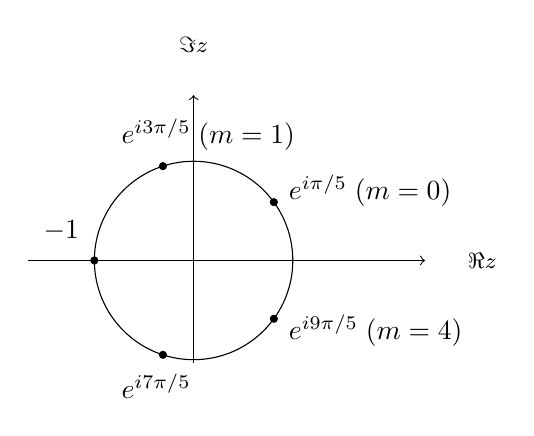
\begin{tikzpicture}[scale=.42]
\draw[->] (-5,0) -- (7,0);
\draw[->] (0,-3.1) -- (0,5);
\node[anchor=west] at (8,0) {\footnotesize $\Re z$};
\node[anchor=south] at (0,6) {\footnotesize $\Im z$};
%\foreach \x in {-5,-4,-3,-2,-1,1,2,3,4,5,6,7,8,9}
%\draw (\x,5pt) -- (\x,-5pt);
%\foreach \y in {-2,-1,1,2,3,4,5,6}
%\draw (5pt,\y) -- (-5pt,\y);
\filldraw (-3,0) circle [radius=3pt] node[anchor=south]{};

\filldraw (3*0.80901699437,3*0.587785252294) circle [radius=3pt] node[anchor=south] {};
\node[anchor=west] at (3.2*0.80901699437,3.6*0.587785252294) {$e^{i\pi/5}\; (m=0)$};
\filldraw (-3*.30901699437,3*0.95105651629) circle [radius=3pt] node[anchor=east] {};
\node[anchor=west] at (-8*.30901699437,4*0.95105651629) {$e^{i3\pi/5}\;(m=1)$};
\node[anchor=south] at (-4,.3) {$-1$};
\filldraw (-3*.30901699437,-3*0.95105651629) circle [radius=3pt] node[anchor=east] {};
\node[anchor=west] at (-8*.30901699437,-4*0.95105651629) {$e^{i7\pi/5}$};
\filldraw (3*0.80901699437,-3*0.587785252294) circle [radius=3pt] node[anchor=south] {};
\node[anchor=west] at (3.2*0.80901699437,-3.6*0.587785252294) {$e^{i9\pi/5}\; (m=4)$};

%\filldraw (3,-3) circle [radius=3pt] node[anchor=north] {$A \V{e}_2$};
%\filldraw (-7,2) circle [radius=3pt] node[anchor=east] {$A \V{u}$};
%\filldraw (9,6) circle [radius=3pt] node[anchor=north] {$A \V{v}$};
%\draw[-] (0,0) to (4,5);
%\node[anchor=south] at (2,3) {\footnotesize $r$};
\draw (3,0) arc (0:360:3);
%\node[anchor=south] at (3.3,1.1) {\footnotesize $\theta$};
%\draw[->,shorten <=4pt,shorten >=4pt] (0,1) to[bend right=30] (3,-3);
%\draw[->,shorten <=4pt,shorten >=4pt] (-1,-2) to[bend right=20] (-7,2);
%\draw[->,shorten <=4pt,shorten >=4pt] (3,2) to[bend left=20] (9,6);
\end{tikzpicture}
\\
{\small \textit{Femterøttene til -1}}
\end{center}
Merk hvordan røttene sprer seg jevnt ut på en sirkel om origo. 
Merk også at om vi lar $m> 4$ eller $m<0$, får vi røtter som allerede er listet opp.
\end{ex}

%\section*{Går alt dette greit?}
%Konstruksjonen av de reelle tallene $\R$ fra de rasjonale tallene $\Q$ er komplisert nok til at selv matematikkstudenter ikke blir plaget særlig med det. 
%Den formelle konstruksjonen av $\C$ fra $\R$ er ikke på langt nær så komplisert, 
%men man trenger fremdeles noen konsepter som ligger noe utenfor det vi kan gjøre i dette kurset.
%
%De reelle tallene er et eksempel på en \emph{ordnet} kropp med addisjon og multiplikasjon. 
%Det at de er ordnet, betyr at man alltid kan avgjøre hvilket av to reelle tall som er størst, 
%og kropp betyr at de tilfredsstiller noen aksiomer som er til forveksling like vektorromsaksiomene, 
%og noen andre aksiomer i tillegg. 
%De komplekse tallene er et eksempel på en kropp som ikke er ordnet, 
%siden man ikke kan si om et komplekst tall er større enn et annet, 
%akkurat som vi ikke i $\R^2$ kan si at en vektor er større enn en annen. 
%(Du kan si at en vektor er lengre enn en annen, men det er ikke noen ordning, 
%for to forskjellige vektorer kan være like lange. 
%To reelle tall er like store kun dersom de er identiske.)

\kapittelslutt
